\thispagestyle{empty}
%----------------------------------------------------------------------
\chapter{Modeling}
\label{modeling.chap}
%----------------------------------------------------------------------

\section{Objectives}
%----------------------------------------------------------------------

The modeling of a system starts with a good description (see Section~\ref{description.sec}). Very often, the system can is made of numerous elements (e.g. cars, particles...) or can be decomposed into small chunks (string, heated body...). In this course we want to obtain PDEs: this means that the dynamics is local. Small elements influence only their neighbors through quantities that are very important: tension and curvature for a string, density and flow for traffic... In order to obtain PDEs, it is often necessary to assume such quantities are slowly varying and that one can \emph{scale} the system. Moreover, one should keep only a very limited number of quantities and simplifying assumptions are key to that objective (neglect gravity, torsion, viscosity...). Finally, an equation (even after scaling) is always obtain as limit of another equation: it is important to explain which principles (physical or other) lead to these equations, be it a conservation equation or dynamical equations.

Now, a model is not complete with only a PDE: initial and boundary conditions must be explicit, the control parameter (or the space of choice) must be given as well as the optimization criteria. The following examples illustrate this method. 

\section{Derivation of partial differential equations}
%----------------------------------------------------------------------
This section shows how one can describe some simple systems and derive from physical principles the PDEs modeling their behavior.

\subsection{2D wave equation}
% ***********************************************************************************
% Pure LaTeX part to be inserted in a document (be careful of depencies of packages & commands
% Prepared by XXX and YYY under the supervision of Arnaud de La Fortelle
% Fall 2017
% 2D wave propagation subsection of the modeling part
% ***********************************************************************************

\subgroup{1}{Bradley Cage and Lin Yang

\paragraph{Description}
\begin{figure}[htb]
	\centering
	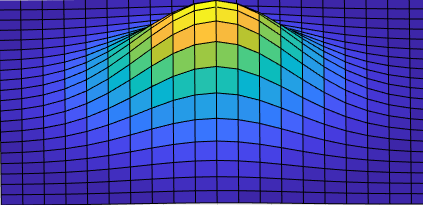
\includegraphics[width=10cm]{Figures/2D_waves_system.png}       
	\caption{The membrane system }
	\label{2D_waves_system.fig}
\end{figure}

Our system is comprised of a flexible membrane stretched to some shape, with all of its edges fixed in place. The desired goal is to understand the vertical position of the various points on the membrane over time. The membrane in this system has vertical deflections which are small compared to its overall size, and deflections happen only in the vertical direction.

This 2D system is a continuation of the 1D wave equation, and is a natural precursor to the 3D wave case. 


\paragraph{Model}
Assumptions:
\begin{itemize}
	\item Membrane has uniform planar density $\rho$
    \item The tension per unit length, $F_t$, caused by stretching the membrane is the same at all points and in all directions and does not change during the motion
    \item Vertical position is given by some function $u(x,y,t)$
\end{itemize}
\begin{figure}[htb]
	\centering
	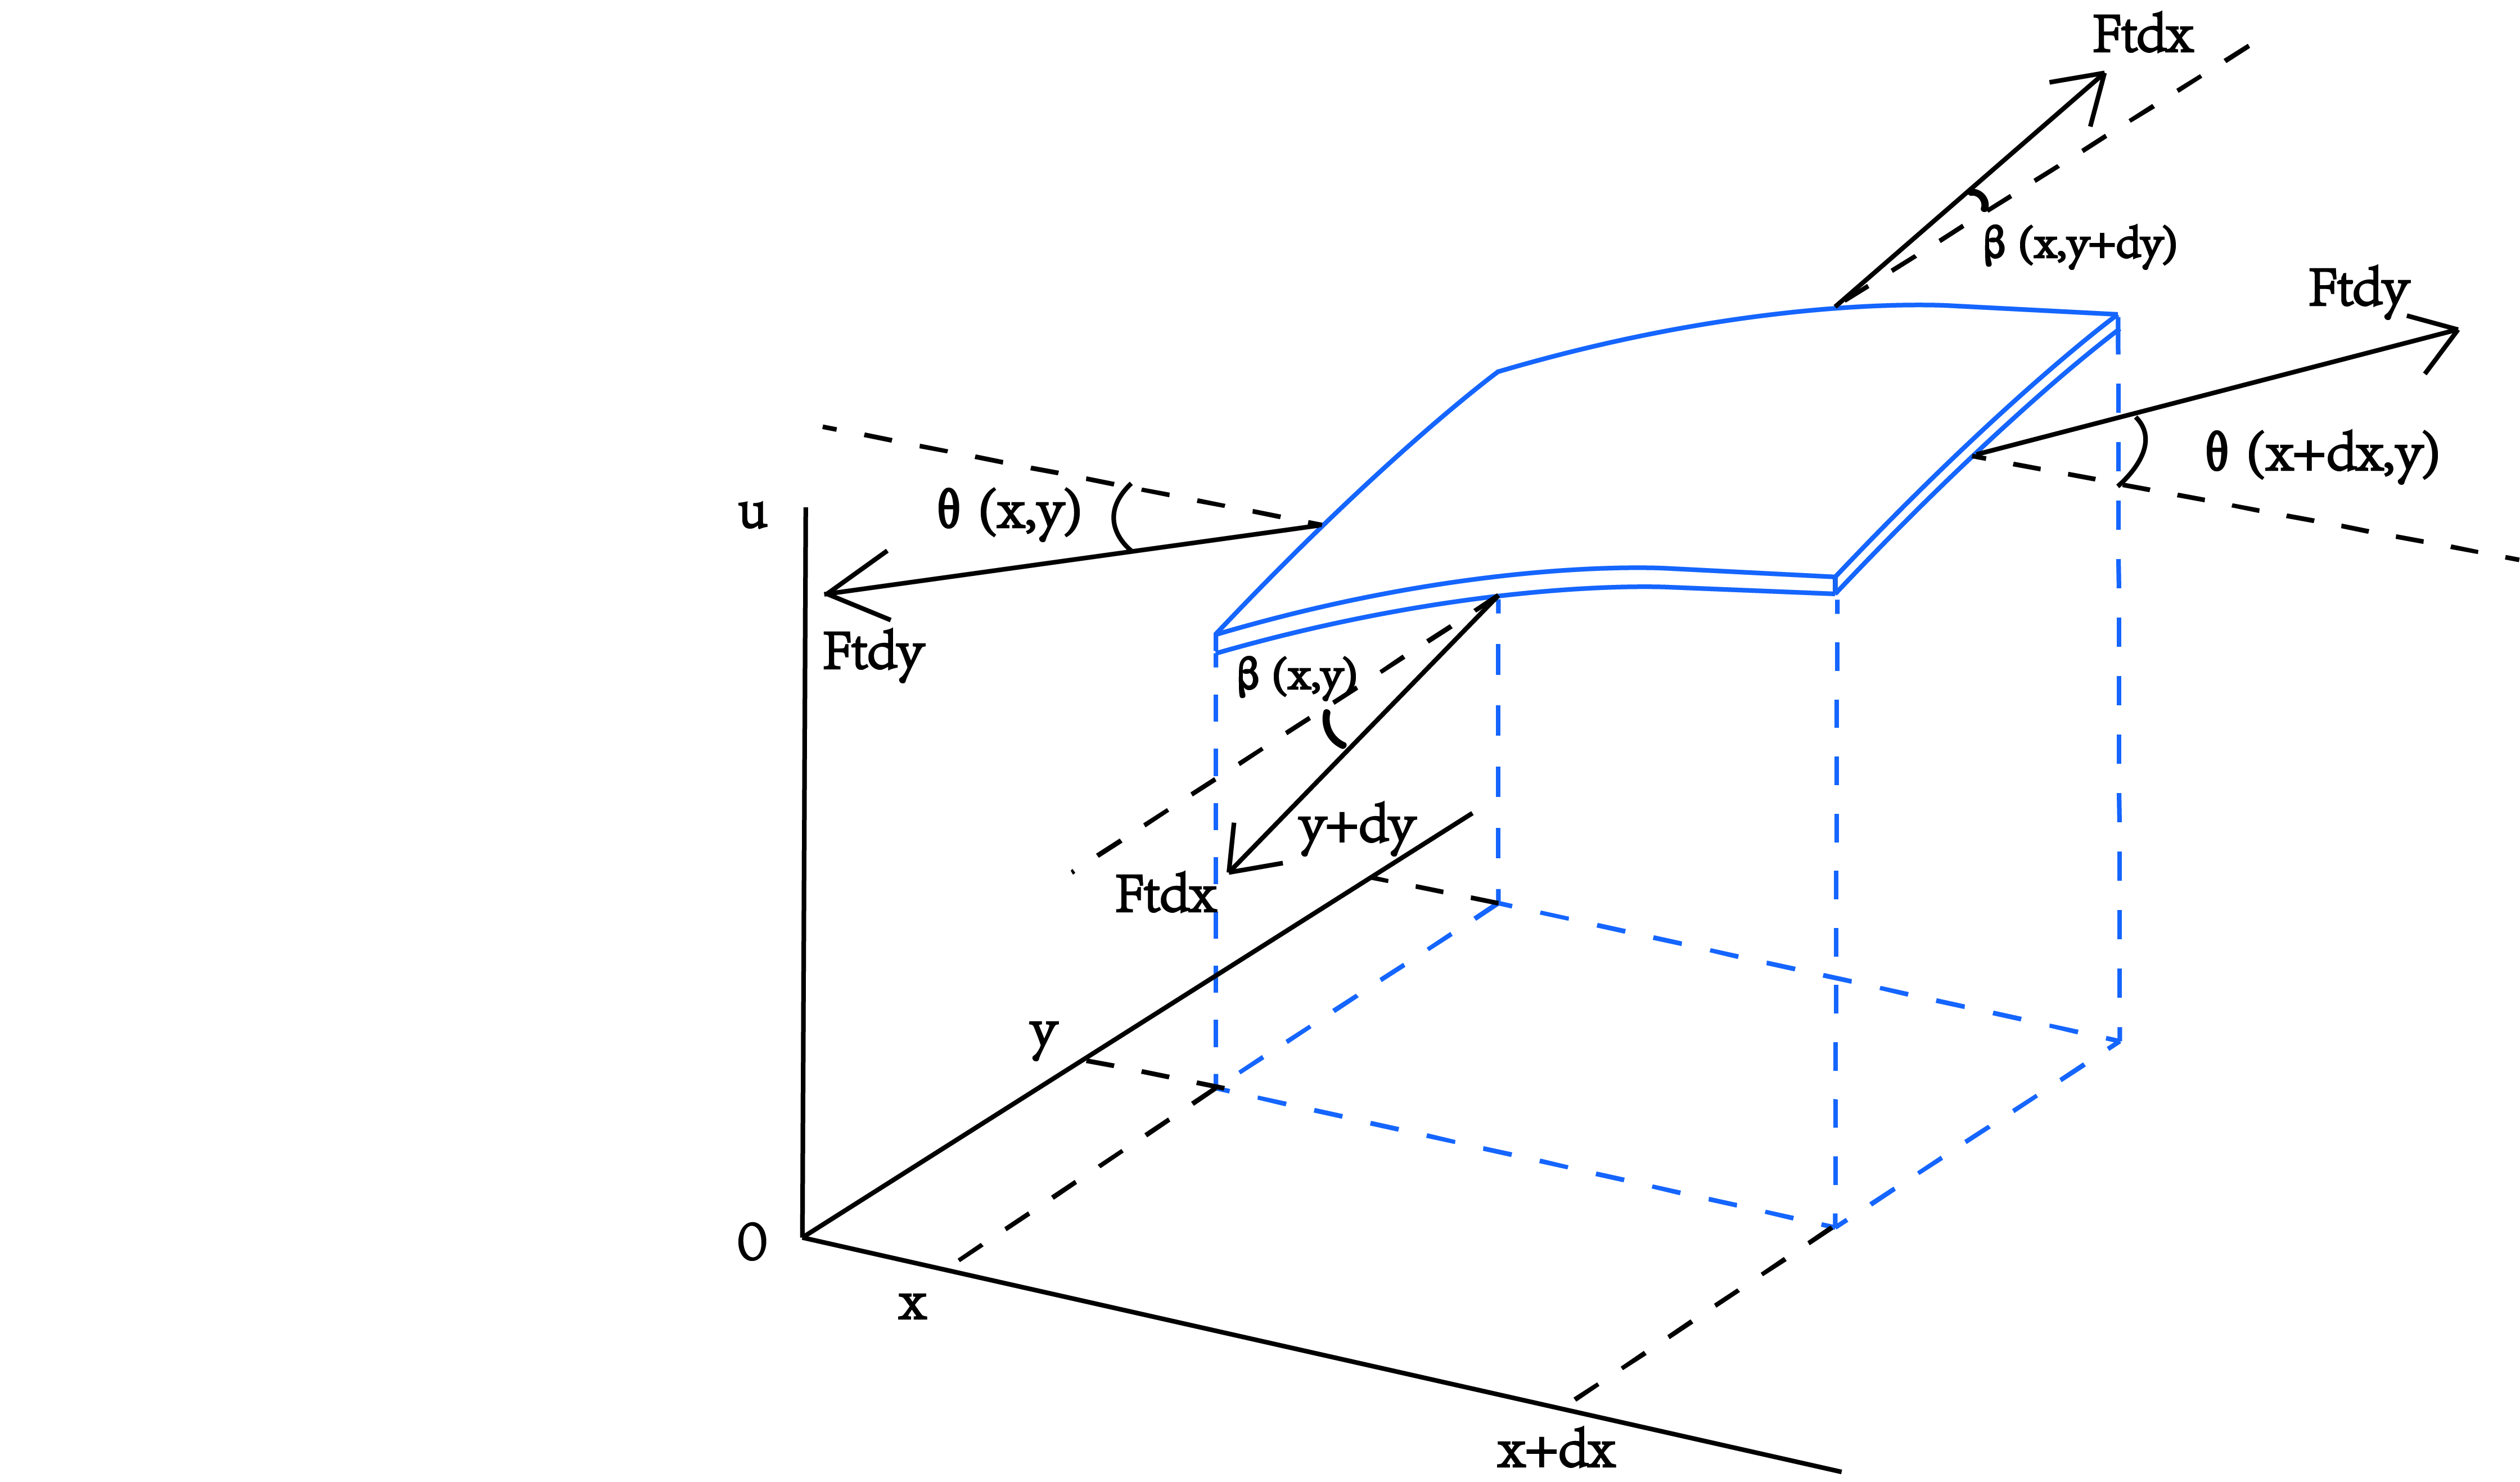
\includegraphics[width=15cm]{Figures/2D_waves_model.png}       
	\caption{The force analysis of a small section of the membrane system }
	\label{2D_waves_model.fig}
\end{figure}
We begin from basic principles.

$$\Sigma F = m\vec{a}$$

\noindent Taking some small section of the membrane $\ud x$ by $\ud y$, we can replace mass and acceleration and since we know density and that $\vec{a}$ is the second derivative of position with respect to time, thus enabling us to rewrite the equation.

\begin{equation}
\label{no_balance}
\Sigma F = \rho \ud x\ud y \frac{\partial^2u}{\partial t^2}
\end{equation}

\noindent Performing a force balance on the section of membrane in the x and y directions gives us tensions at each on each side, then resolved to their vertical components. Remember that since tension is constant per unit length, we must multiply the force acting on each side by the length of that side. Thus, the force acting on this balance lets us rewrite $\Sigma F$ (that is we only consider vertical forces, forces acting in the $x-u$ and $y-u$ planes): 

$$\Sigma F = F_x + F_y$$

$$F_x = F_t\ud y\Big[\sin\big( \theta (x+\ud x,y,t) \big) - \sin \big((\theta (x,y,t)\big)\Big]$$
$$F_y = F_t\ud x\Big[\sin\big( \beta (x,y+\ud y,t) \big) - \sin \big((\beta (x,y,t)\big)\Big]$$

\noindent We can confidently use the small angle approximation $\sin$ in the x direction

$$ \sin(\theta) \approx \tan(\theta) = \frac{\partial u}{\partial x} = u_x$$

\noindent and likewise in the y direction 

$$ \sin(\beta) \approx \tan(\beta) = \frac{\partial u}{\partial y} = u_y$$

\noindent to get our equations into the form

$$F_x = F_t\u dy\Big[u_x(x+\ud x,y,t) - u_x(x,y,t)\Big]$$
$$F_y = F_t\u dx\Big[u_y(x,y+\ud y,t) - u_y(x,y,t)\Big]$$

\noindent From there we can sum these forces and plug them back in to equation \ref{no_balance}

$$\rho \ud x\ud y \frac{\partial^2u}{\partial t^2} = F_t\bigg[dy\Big[u_x(x+\ud x,y,t) - u_x(x,y,t)\Big]+dx\Big[u_y(x,y+\ud y,t) - u_y(x,y,t)\Big] \bigg]$$

\noindent We then divide by $\ud x$ and $\ud y$ and take the limit as $\ud x,\ud y \to 0$:

$$\rho\frac{\partial^2u}{\partial t^2} = \lim_{\ud x,\ud y\to 0} F_t \bigg[ \frac{u_x(x+\ud x,y,t) - u_x(x,y,t)}{\ud x} + \frac{u_y(x,y+\ud y,t) - u_y(x,y,t)}{\ud y} \bigg]$$

\noindent We recognize that we now have derivatives in the form of difference quotients, and can take the partial derivative of each one (since $u$ is a function of multiple variables)

\begin{equation}
\rho \frac{\partial^2u}{\partial t^2} = F_t\bigg[\frac{\partial}{\partial x}u_x + \frac{\partial}{\partial y}u_y \bigg] = F_t\bigg[\frac{\partial^2 u}{\partial x^2} + \frac{\partial^2 u}{\partial y^2}\bigg]
\end{equation}

\noindent Dividing over the uniform  tension, we reach our final form.

\begin{equation}
\frac{\rho}{F_t}\frac{\partial^2u}{\partial t^2} = \frac{\partial^2 u}{\partial x^2} + \frac{\partial^2 u}{\partial y^2}
\end{equation}

\noindent We can adhere to standard conventions and write our final 2D wave equation as 


\begin{align}
a^2 \frac{\partial^2u}{\partial t^2} &= \frac{\partial^2 u}{\partial x^2} + \frac{\partial^2 u}{\partial y^2} & a &= \sqrt{\frac{\rho}{F_t}}
\label{final_eq}
\end{align}

\noindent Equation \ref{final_eq} is also commonly written using the Laplace operator:

\begin{equation}
a^2 \frac{\partial^2u}{\partial t^2} = \nabla^2 u
\end{equation}
\noindent Initial condition:
\begin{itemize}
	\item When t=0, the vertical position all over the membrane is 0, i.e., $u(x,y,0)=0$.
\end{itemize}
\begin{figure}[htb]
	\centering
	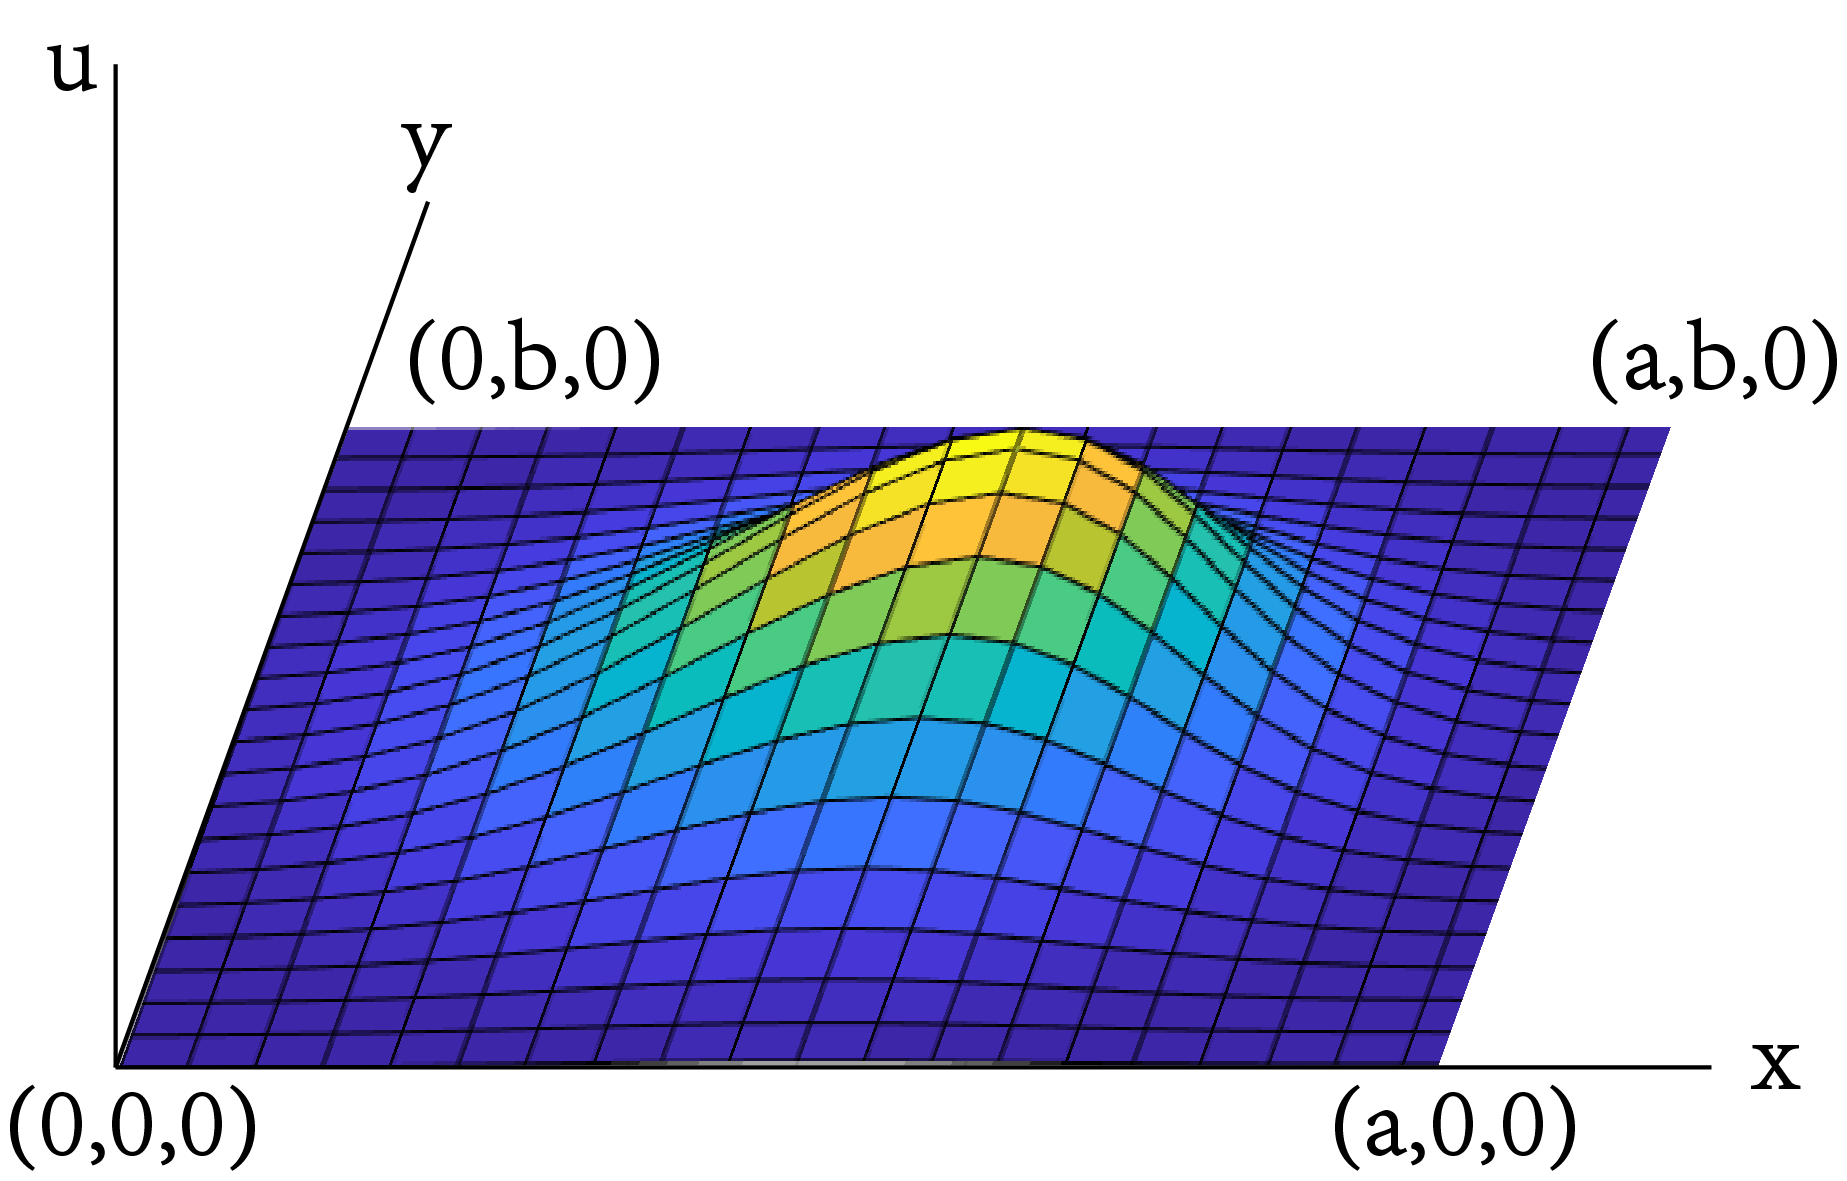
\includegraphics[width=10cm]{Figures/2D_waves_boundary_conditions.png}       
	\caption{The membrane system's boundaries}
	\label{2D_waves_boundary_conditions.fig}
\end{figure}
Boundary condition:
\begin{itemize}
	\item The vertical positions of the 4 edges of the membrane remain 0 all the time, i.e., $u(x,0,t)=0$, $u(0,y,t)=0$, $u(a,y,t)=0$, $u(x,b,t)=0$.
\end{itemize}
\noindent Some hints for the control and the cost function of the 2D wave equation:
\begin{itemize}
	\item Control: Maintain the highest vertical deflection of the membrane to be some constant height H   
    \item The cost function then could be finding the smallest force exerted on the membrane to maintain the highest height H in the membrane system
    
\end{itemize}

\subsection{2D heat diffusion}
% ***********************************************************************************
% Pure LaTeX part to be inserted in a document (be careful of depencies of packages & commands)
% Prepared by Qingan Zhao and Ruitong Zhu under the supervision of Arnaud de La Fortelle
% Fall 2017
% 2D heat diffusion subsection of the modeling part
% ***********************************************************************************

\subgroup{2}{Qingan Zhao and Ruitong Zhu}

\paragraph{Description}
The aim of this part is to describe and model a PDE that describes temperature dynamics in a two-dimensional body via heat conduction.
Basically, heat conduction is the exchange of heat from regions of higher temperatures into regions with lower temperatures, which varies in the transfer rate for different materials.

Consider a thin flat body with a constant thickness $h$ and uniform density $\rho'$. Assume that the faces of the thin body are in perfect insulation, which means there is no heat flow travel in the out-of-plane direction of the body. Hence, heat can only flow in the direction within the plane of the body, which turns into a two-dimensional problem. Then a two-dimensional coordinate system is established such that each point of the body can be described with a coordinate $(x,y)$. Then the (2D-uniform) density of the body is $\rho = \rho' h$. Denote the temperature function of each point by $T$ so that the temperature of the body at position $(x,y)$ and time $t$ are described as $T(x,y,t)$, as shown in Figure~\ref{heatSystem.fig}. The goal is to derive $T(x,y,t)$ when there is no internal heat source.
\begin{figure}[htb]
	\centering
	\includegraphics[width=10cm]{heatSystem.pdf}       
	\caption{System description in 2 dimensions}\label{heatSystem.fig}
\end{figure}

\paragraph{Model}
Consider a small rectangular element of the body with vertices $(x,y)$, $(x+\ud x,y)$, $(x, y+\ud y)$, and $(x+\ud x, y+\ud y)$. The heat flows are shown in Figure~\ref{heatElement.fig}.
\begin{figure}[htb]
	\centering
	\includegraphics[width=8cm]{HeatElement.pdf}       
	\caption{Heat flows in a small rectangular element of the body}\label{heatElement.fig}
\end{figure}

The heat amount $Q$ (i.e the thermal energy) of the rectangular element at time $t$ is: 
\begin{equation}
Q(x,y,t)=C m T(x,y,t)
\end{equation}
where $C$ is called \emph{heat capacity}, which is a supposed to be constant (assuming the material is uniform and temperature do not vary too much); $m = \rho A$ is the mass of the rectangular element where $A$ its surface.

The rate of thermal energy change with respect to time is therefore:
\begin{equation}\label{thermalEnergyChange.eq}
\frac{\partial Q}{\partial t} = C\rho \ud x \ud y\frac{\partial T}{\partial t}
\end{equation}

As shown in Figure~\ref{heatElement.fig}, the incoming flow is $F_1 + F_2 + F_3 + F_4$. Denote the heat flux $\vec q$ in horizontal and vertical directions by $q_x$ and $q_y$, then we have:
\begin{eqnarray} 
F_1 &=& q_x(x,y,t)\ud y\label{flow1}\\
F_2 &=& -q_y(x,y+\ud y,t)\ud x\label{flow2}\\
F_3 &=& q_y(x,y,t)\ud x\label{flow3}\\
F_4 &=& -q_x(x+\ud x,y,t)\ud y\label{flow4}
\end{eqnarray}

Now, we know that according to energy conservation, the thermal energy variation of any small element (as in Equation~(\ref{thermalEnergyChange.eq})) is equal to the total incoming heat flow.  By putting the partial flows as in Equations~(\ref{flow1})-(\ref{flow4}), this conservation principle yields:
\begin{equation}\label{thermalEnergyChange.eq2}
C\rho \ud x \ud y\frac{\partial T}{\partial t} = \ud y [q_x(x,y,t)-q_x(x+\ud x,y,t)]+\ud xh[q_y(x,y,t)-q_y(x,y+\ud y,t)]
\end{equation}

Now, another physical principle, \emph{Fourier's Law}, states that the heat flow is (negatively) proportional to the gradient of temperature:
\begin{equation}\label{FourierLaw.eq}
\vec q = -k\nabla T
\end{equation}
where $k$ is known as the thermal conductivity of the material (also considered as a constant). Then $q_x$ and $q_y$ are expressed as:
\begin{equation}
\begin{split}
q_x=-k\frac{\partial T}{\partial x}\\
q_y=-k\frac{\partial T}{\partial y}
\end{split}
\end{equation}

Hence, Equation~(\ref{thermalEnergyChange.eq2}) can be written as:
\begin{equation}\label{thermalEnergyChange.eq3}
\frac{\partial Q}{\partial t}=k\ud yh\left(\frac{\partial T(x+\ud x,y,t)}{\partial x}-\frac{\partial T(x,y,t)}{\partial x}\right)+k\ud xh\left(\frac{\partial T(x,y+\ud y,t)}{\partial y}-\frac{\partial T(x,y,t)}{\partial y}\right)
\end{equation}

Combine Equation~(\ref{thermalEnergyChange.eq}) and~(\ref{thermalEnergyChange.eq3}):
\begin{equation}
\frac{\partial T(x,y,t)}{\partial t}=\frac{k}{c\rho}\left(\frac{\partial ^2 T(x,y,t)}{\partial x^2}+\frac{\partial ^2 T(x,y,t)}{\partial y^2}\right)
\end{equation}

Denote $k/c\rho$ by $a^2$, and the two-dimensional heat equation can be drawn:
\begin{equation}
\frac{\partial T}{\partial t}=a^2\left(\frac{\partial ^2 T}{\partial x^2}+\frac{\partial ^2 T}{\partial y^2}\right)
\end{equation}

If we would like to solve the PDE in practice, the initial conditions and (or) boundary conditions need to be specified. For initial conditions, assume that in domain $\Omega$:
\begin{equation}
T(x,y,0)=\phi(x,y) 
\end{equation}

As for boundary conditions, we should know either the value or the gradient of the function at some boundaries (i.e., fixed temperature or fixed flow).

For fixed temperature, for example, at the boundary $x=0$, a boundary condition could be stated as follow:
\begin{equation}
T(0, y, t)=0
\end{equation}  
such a boundary condition means the temperature will always be $0$ at the line $x=0$ of the 2D plane.

The boundary condition could aslo be a fixed flow. For example, at the boundary $x=0$:
\begin{equation}
\nabla (0, y, t)=0
\end{equation}
such a boundary condition means that there is no heat transfer at the line $x=0$ of the 2D plane.

When the conditions are given, it is the time to solve the PDE. Most simple PDEs can be solved using analytical methods, such as separation of variables and transform techniques. If the analytical methods do not work, numerical methods can be implemented to find the numerical approximations to the solutions of the PDE. A practical example with boundary conditions will be given in Section 2.3, where the analytical solution will be derived.

Once a system has been solved, we could enhance it by implementing the optimization. One thing we could do is to add some controls. For example, we would like the temperature of a plane less as stable as possible. A proper cost function could be a mathematical expression giving $\ud T/\ud t$ as a function of the external heat sourse. Tools such as Kalman filter can be implemented to do the optimization. A real world example is in aircraft temperature monitoring, for which temperature changes that above a threshold should be warned. 



\subsection{2D random walk}
% ***********************************************************************************
% Pure LaTeX part to be inserted in a document (be careful of depencies of packages & commands
% Prepared by XXX and YYY under the supervision of Arnaud de La Fortelle
% Fall 2017
% 2D wave propagation subsection of the modeling part
% ***********************************************************************************

\subgroup{4}{Carlin Liao}

\paragraph{Description}
Consider a particle in a discrete two-dimensional grid at location $\vec{x}=[x_1,x_2]$ that moves in discrete time intervals. On each movement, the particle has an equal probability of moving one unit in any of the four cardinal directions $[x_1+1,x_2]$, $[x_1-1,x_2]$, $[x_1,x_2+1]$, and $[x_1,x_2-1]$. Our goal is to describe the probability of the point arriving at point $\vec{x}$ at time $t+1$, $P[\vec{x},t+1]$ using Fick's Law.

% \usepackage{tikz}
\begin{figure}[htb]
\centering
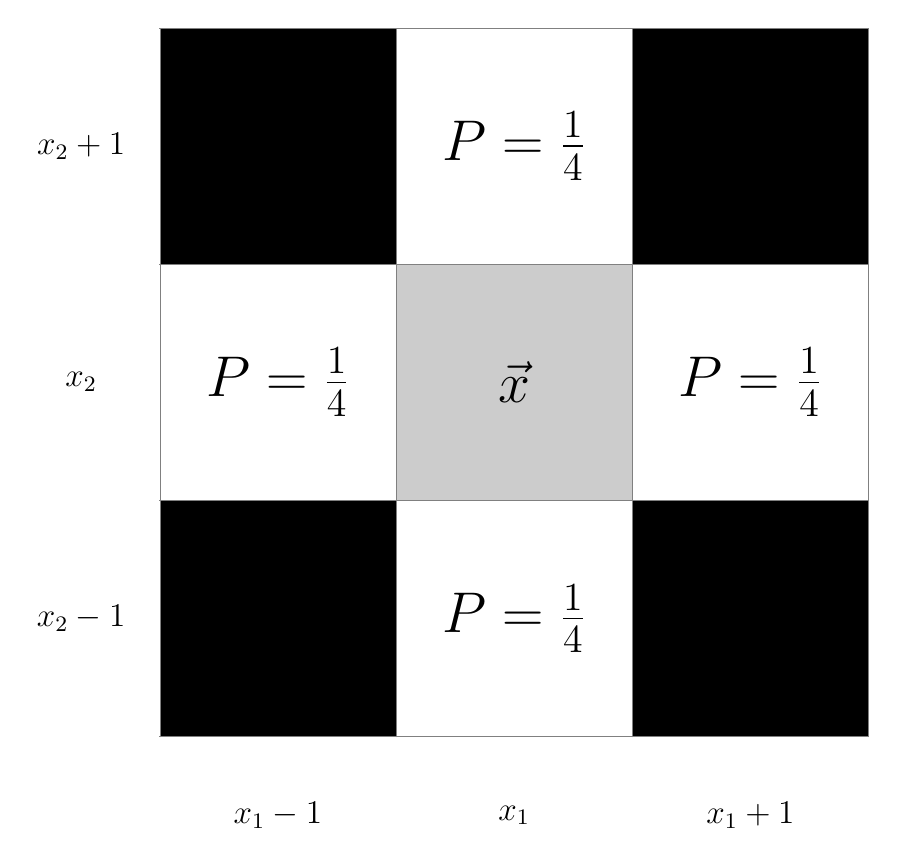
\begin{tikzpicture}

\fill[black] (-3,-3) rectangle (0,0);
\fill[black] (3,3) rectangle (6,6);
\fill[black] (-3,3) rectangle (0,6);
\fill[black] (3,-3) rectangle (6,0);
\fill[gray!40!white] (0,0) rectangle (3,3);

\draw[step=3cm,gray,very thin] (-3.01,-3.01) grid (6,6);

% \node at (1.5,1.5) {\huge$(x_1,x_2)$};
\node at (1.5,1.5) {\huge$\vec{x}$};
\node at (-1.5,1.5) {\huge$P=\frac{1}{4}$};
\node at (1.5,-1.5) {\huge$P=\frac{1}{4}$};
\node at (1.5,4.5) {\huge$P=\frac{1}{4}$};
\node at (4.5,1.5) {\huge$P=\frac{1}{4}$};

\node at (-4,4.5) {\large\bf$x_2+1$};
\node at (-4,1.5) {\large\bf$x_2$};
\node at (-4,-1.5) {\large\bf$x_2-1$};

\node at (-1.5,-4) {\large\bf$x_1-1$};
\node at (1.5,-4) {\large\bf$x_1$};
\node at (4.5,-4) {\large\bf$x_1+1$};

\end{tikzpicture}
\caption{Probability of next step in the 2D random walk}\label{2DrandomWalkProbs.fig}
\end{figure}
    
\paragraph{Model}
Ultimately, our goal is to find a form of Fick's Law using $p(\vec{x},t) = P[\vec{x},t]$, of which the above description is setup for. Note that we can replace $t$ with $t+1$ or any other $t$ without loss of generality due to the memoryless property of 2D random walk.

We begin by describing $P[\vec{x},t+1]$ using our knowledge of the probabilities of where it may be at the prior time step $t$.

\begin{align*}
    P\left[\vec{x}, t+1\right] =&\quad\, \frac{1}{4}P\left[\begin{bmatrix} x_1+1\\x_2 \end{bmatrix}, t\right]\\
    &+\frac{1}{4}P\left[\begin{bmatrix} x_1-1\\x_2 \end{bmatrix}, t\right]\\
    &+\frac{1}{4}P\left[\begin{bmatrix} x_1\\x_2+1 \end{bmatrix}, t\right]\\
    &+\frac{1}{4}P\left[\begin{bmatrix} x_1\\x_2-1 \end{bmatrix}, t\right]
\end{align*}

In order to develop the parallels to Fick's law, we take the Taylor expansions of each of our probabilities with respect to $t$ for $P\left[\vec{x}, t+1\right]$ and with respect to $x$ for each of the probabilities we've used at time $t$.

First, we take the our target probability and find its first order Taylor expansion with respect to time, and using our $p(\vec{x},t)$ as described earlier.
\begin{align*}
    P\left[\vec{x}, t+1\right] &\approx P\left[\vec{x}, t+1\right] + \nabla^T_t\left(P\left[\vec{x}, t+1\right]\right) (t+1-t) \\
    &= p + \frac{\partial p}{\partial t} \\
    &= p
\end{align*}
Note that we exploit the memoryless property of random walk to reduce $\frac{\partial p}{\partial t}$ to 0, as the probability that a particle performing truly random walk is in a certain location in space is not influenced by time.

Next, we take the second order Taylor expansion of our probabilities of movement in the $x_1$ direction, using similar substitutions as before. Here, $\mathcal{H}(f)$ describes the Hessian of the function $f$. 
\begin{align*}
    P\left[\begin{bmatrix} x_1\pm1\\x_2 \end{bmatrix}, t\right] &\approx p + \nabla^T_{\vec{x}}(p) \left(\begin{bmatrix} x_1\pm1\\x_2 \end{bmatrix} - \vec{x}\right) + \left(\begin{bmatrix} x_1\pm1\\x_2 \end{bmatrix} - \vec{x}\right)^T \mathcal{H}(p)  \left(\begin{bmatrix} x_1\pm1\\x_2 \end{bmatrix} - \vec{x}\right) \\
    &= p + \left(\frac{\partial p}{\partial x}\right)^T \begin{bmatrix} \pm1\\0 \end{bmatrix} + \begin{bmatrix} \pm1\\0 \end{bmatrix}^T \begin{bmatrix}
        \frac{\partial^2 p}{\partial x_1^2} & \frac{\partial p}{\partial x_2 x_1} \\
        \frac{\partial p}{\partial x_1 x_2} & \frac{\partial^2 p}{\partial x_2^2}
    \end{bmatrix} \begin{bmatrix} \pm1\\0 \end{bmatrix} \\
    &= p \pm \left(\frac{\partial p}{\partial x}\right)^T \begin{bmatrix} 1\\0 \end{bmatrix} + \frac{\partial^2 p}{\partial x_1^2}
\end{align*}

Similarly, we take the second order Taylor expansion for probabilities in the $x_2$ direction.
\begin{align*}
    P\left[\begin{bmatrix} x_1\\x_2\pm1 \end{bmatrix}, t\right] &\approx 
    p + 
    \nabla^T_{\vec{x}}(p) \left(\begin{bmatrix} x_1\\x_2\pm1 \end{bmatrix} - \vec{x}\right) + \left(\begin{bmatrix} x_1\\x_2\pm1 \end{bmatrix} - \vec{x}\right)^T \mathcal{H}(p)  \left(\begin{bmatrix} x_1\\x_2\pm1 \end{bmatrix} - \vec{x}\right) \\
    &= p \pm \left(\frac{\partial p}{\partial x}\right)^T \begin{bmatrix} 0\\1 \end{bmatrix} + \begin{bmatrix} 0\\1 \end{bmatrix}^T \begin{bmatrix}
        \frac{\partial^2 p}{\partial x_1^2} & \frac{\partial p}{\partial x_2 x_1} \\
        \frac{\partial p}{\partial x_1 x_2} & \frac{\partial^2 p}{\partial x_2^2}
    \end{bmatrix} \begin{bmatrix} 0\\1 \end{bmatrix} \\
    &= p \pm \left(\frac{\partial p}{\partial x}\right)^T \begin{bmatrix} 0\\1 \end{bmatrix} + \frac{\partial^2 p}{\partial x_2^2}
\end{align*}

Now, we combine all of the above into our original expression
\begin{align*}
    p =&\quad\, \frac{1}{4}\left(p + \left(\frac{\partial p}{\partial x}\right)^T \begin{bmatrix} 1\\0 \end{bmatrix} + \frac{\partial^2 p}{\partial x_1^2}\right)\\
    &+\frac{1}{4}\left(p - \left(\frac{\partial p}{\partial x}\right)^T \begin{bmatrix} 1\\0 \end{bmatrix} + \frac{\partial^2 p}{\partial x_1^2}\right)\\
    &+\frac{1}{4}\left(p + \left(\frac{\partial p}{\partial x}\right)^T \begin{bmatrix} 0\\1 \end{bmatrix} + \frac{\partial^2 p}{\partial x_2^2}\right)\\
    &+\frac{1}{4}\left(p - \left(\frac{\partial p}{\partial x}\right)^T \begin{bmatrix} 0\\1 \end{bmatrix} + \frac{\partial^2 p}{\partial x_2^2}\right)
\end{align*}
We note how the first order terms cancel out and proceed to further simplify. Take note of the use of the Laplacian operator $\nabla^2$.
\begin{align*}
    p &= p + \frac{1}{4}\left(\frac{\partial^2 p}{\partial x_1^2}+\frac{\partial^2 p}{\partial x_1^2}+\frac{\partial^2 p}{\partial x_2^2}+\frac{\partial^2 p}{\partial x_2^2}\right) \\
    0 &= \frac{1}{2}\left(\frac{\partial^2 p}{\partial x_1^2}+\frac{\partial^2 p}{\partial x_2^2}\right)\\
    \nabla^2 p &= \frac{\partial^2 p}{\partial x_1^2}+\frac{\partial^2 p}{\partial x_2^2}\\
    \nabla^2 p &= 0
\end{align*}
We note that this final result to be (as expected) the solution to Fick's second law in the special case of the diffusion (or random walk, in our case) being independent of time, also known as Laplace's equation. For a more general result (i.e. not assuming that our particle's position is independent of time), using these same methods we would arrive at the more general statement of Fick's second law
$$\frac{\partial p}{\partial t} = \nabla^2 p$$

To close, while this result was derived for the two-dimensional random walk case, the derivation for n-dimensions should be readily apparent from this case.


\vspace{12pt}


{\it Adapted in part from} \url{http://engineering.dartmouth.edu/~d30345d/courses/engs43/chapter2.pdf}

\subsection{Heavy chain}

\subgroup{4}{Rob Ruigrok}

\paragraph{Description}
This chapter will cover the derivation of the dynamics of a heavy chain with uniform density $\rho$, length $L$ and a point mass on the end with mass $m$. The top of the chain will be suspended on a rolling trolley, where the lateral speed can be controlled. First, we will derive the dynamics, and later go into more detail on the "flatness" of the system and several control inputs.

\paragraph{Model}

An overview of the system is provided in figure \ref{fig:heavychainoverview}. Let $x$ be coordinate along the length of the chain, where the chain is attached to the trolley at $x=L$. The lateral displacement of the chain is denoted by $y(x,t)$. The problem can be made more complex by adding a point mass $m$ to the end of the chain.

\begin{figure}[h]
\label{fig:heavychainoverview}
\centering
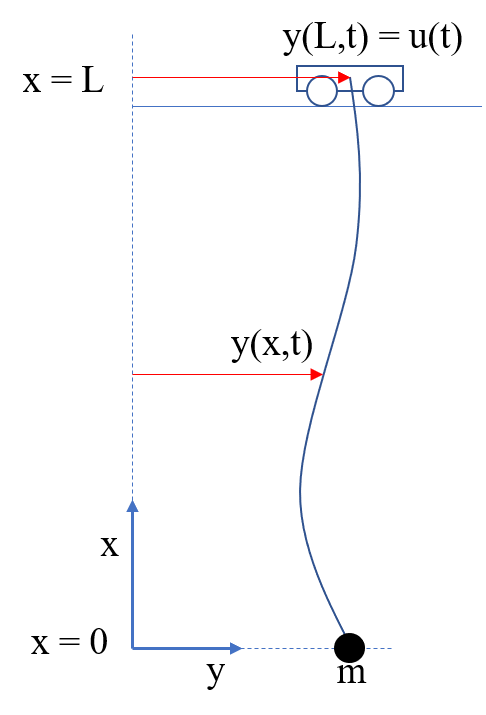
\includegraphics[width = 4cm]{Overview.png}
\end{figure}

The derivation of the dynamics goes largely the same as the derivation of the vibrating spring. Here, however, the tension in the chain will be depending on $x$, and there will now be different boundary conditions linked to the trolley at the top and the attached mass at the bottom. Figure \ref{fig:heavychaindx} illustrates the forces acting on a finite chain element of length $dx$, which is the basis in the derivation of the PDE.\newline

\begin{figure}[h]
\label{fig:heavychaindx}
\centering
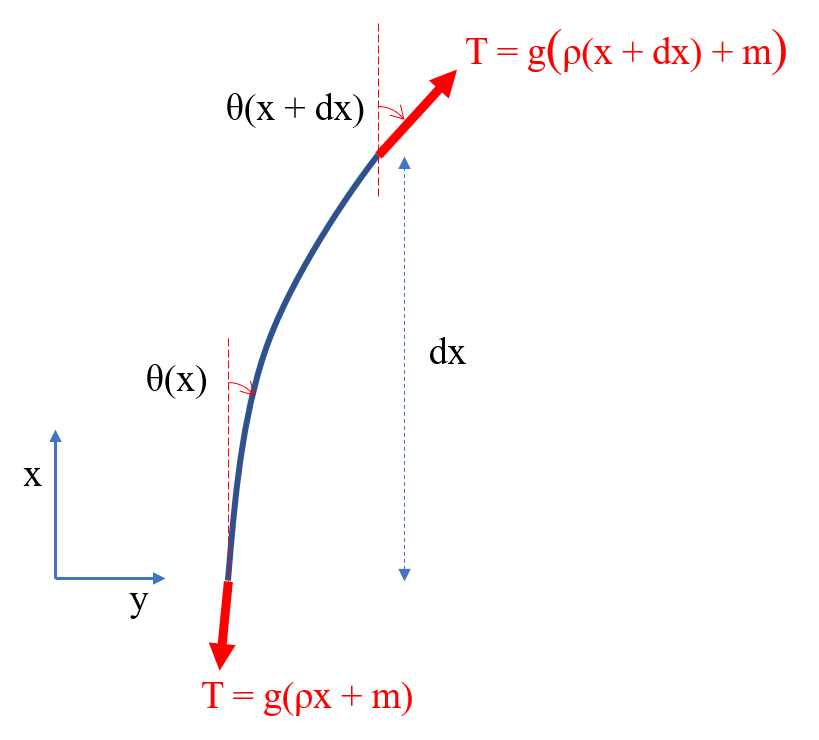
\includegraphics[width = 5cm]{SmallElement.png}
\end{figure}

We start with defining the tension in the chain as a function of $x$:

\begin{equation}
\label{eq:chaintension}
T = (m + x\rho)g
\end{equation}

To analyze the dynamics, we are interested of the lateral component of this tension. When examining an infinitesimal chain element of length $\Delta x$, we are interested in the net lateral force. Instead of defining the force on both sides of element $\Delta x$, we here determining the difference by using a first order Taylor approximation, together with a small angle approximation:

\begin{equation}
\label{eq:chainapprox}
sin(\theta)T \approx tan(\theta)T = \frac{\partial y}{\partial x}T
\end{equation}

\begin{equation}
\label{eq:chainforce}
\Delta F \approx F_x \Delta x = \big[\frac{\partial y}{\partial x}T\big]_x \Delta x
\end{equation}

The lateral motion of an infinitesimal chain element can now be described with Newtons second law of motion, $F = ma$, for which the net force is defined in equation \ref{eq:chainforce}. The mass of the chain element is $\rho \Delta x$, and the acceleration is $\frac{\partial^2 y}{\partial t^2}$

\begin{equation}
\begin{aligned}
    F &= ma \\
    \big[\frac{\partial y}{\partial x}T\big]_x \Delta x &= \rho \Delta x \frac{\partial^2 y}{\partial t^2} \\
    \big[\frac{\partial y}{\partial x} (m + x\rho)g \big]_x &= \rho \frac{\partial^2 y}{\partial t^2}
\end{aligned}
\end{equation}

When there is no mass suspended to end of the chain, the dynamics can be further written out:

\begin{eqnarray}
\label{eq:chainPDE}
    \big[\frac{\partial y}{\partial x} x \rho g \big]_x &=& \rho \frac{\partial^2 y}{\partial t^2} \\
    g \big[\frac{\partial y}{\partial x} x \big]_x &=& \frac{\partial^2 y}{\partial t^2} \\
    g \big[x \frac{\partial^2 y}{\partial x^2} + \frac{\partial y}{\partial x} \big] &=& \frac{\partial^2 y}{\partial t^2}
\end{eqnarray}
with boundary condition: $y(L,t) = u(t) $.


\paragraph{Solving the PDE}
\bigskip
\emph{\textbf{TODO: move part of it to control section
}}\bigskip

It is difficult to directly find a solution for the partial differential equation in equation~5\ref{eq:chainPDE}). For this particular problem, we assume that we know that we can rewrite to a Bessel function. Bessel functions are mainly used to describe wave propagation, and have the following format, where $\alpha$ denotes the order of the Bessel function:

\begin{equation}
\label{eq:Bessels}
x^2\frac{d^2 y}{dx^2} + x\frac{dy}{dx} + (x^2 - \alpha^2)y = 0
\end{equation}

In order to make the formulation in equation \ref{eq:chainPDE} fit this a zero-order Bessel function, we have to do certain changes of variables and convert the problem to the Laplace domain. In the Laplace domain, we can find solutions for our type of Bessel function, after which we need to transform it back to the time domain and reverse the variable changes. \newline

\paragraph{Step 1: substitution}

First step, do a substitution with $p = 2\sqrt{\frac{x}{g}}$. This will change the dependency from y(x,t) to y(p,t). Use the chain rule and find fill out the new values:

\begin{equation}
\label{eq:ChainRule}
\begin{aligned}
\frac{\partial p}{\partial x} &= \frac{1}{g}\bigg(\frac{x}{g}\bigg)^{-\frac{1}{2}} = \frac{1}{g\sqrt{\frac{x}{g}}} = \frac{2}{gp}\\
\frac{\partial y}{\partial x} &=  \frac{\partial y}{\partial p} \frac{\partial p}{\partial x} + \frac{\partial y}{\partial t} \cancelto{0}{\frac{\partial t}{\partial x}} = \frac{\partial y}{\partial p} \frac{2}{gp}
\end{aligned}
\end{equation}

When we fill everything out in the left part of equation \ref{eq:chainPDE}, we get the following expression:

\begin{equation}
\label{eq:chaincombination1}
\begin{aligned}
g \frac{\partial}{\partial x}\big[\frac{\partial y}{\partial x} x \big] &= g \frac{\partial}{\partial x}\big[\frac{\partial y}{\partial p} \frac{2}{gp} \frac{1}{4}gp^2 \big] = g \frac{\partial}{\partial x}\big[\frac{\partial y}{\partial p} \frac{p}{2} \big] \\
&= g \frac{\partial}{\partial p}\big[\frac{\partial y}{\partial p} \frac{p}{2} \big]\frac{\partial p}{\partial x} = g \big[\frac{\partial^2 y}{\partial p^2} \frac{p}{2} + \frac{1}{2} \frac{\partial y}{\partial p}\big] \frac{2}{gp} \\
&= \frac{\partial^2 y}{\partial p^2} + \frac{1}{p} \frac{\partial y}{\partial p}
\end{aligned}
\end{equation}

So the total equation can be written as:
\begin{eqnarray}
\label{eq:chaincombination2}
 g \big[\frac{\partial y}{\partial x} x \big]_x - \frac{\partial^2 y}{\partial t^2} &=& 0 \\
  \frac{\partial^2 y}{\partial p^2} + \frac{1}{p} \frac{\partial y}{\partial p} - \frac{\partial^2 y}{\partial t^2} &=& 0 \\
 p \frac{\partial^2 y}{\partial p^2} +
  \frac{\partial y}{\partial p} - p \frac{\partial^2 y}{\partial t^2} &=& 0
\end{eqnarray}

\paragraph{Step 2: transform to Laplace domain}

When converting the from the time domain, we use the following notation:
\begin{center}
$y(x,t) \xrightarrow{\mathcal{L}} Y(x,s)$
\end{center}
Further, to get the Laplace transform in the desired format, we require that the systems is initially \textit{at rest}, which means that $y(x,0)=0$ and $\dot{y}(x,0)=0$.

\begin{equation}
\label{eq:heavychainlaplace}
\begin{aligned}
 p \frac{\partial^2 y(x,t)}{\partial p^2} +
  \frac{\partial (x,t)}{\partial p} - p \frac{\partial^2 y(x,t)}{\partial t^2} = 0 \\
  \xrightarrow{\mathcal{L}}
 p \frac{\partial^2 Y(x,s)}{\partial p^2} +
  \frac{\partial Y(x,s)}{\partial p} - p s^2 Y(x,s) = 0
\end{aligned}
\end{equation}

NEW CHANGE OF VARIABLES (did it myself on paper, still need to isert)\newline
Bessel function!




\section{Manipulation of partial differential equations}
%----------------------------------------------------------------------

\subsection{Weak formulation}
% ***********************************************************************************
% Pure LaTeX part to be inserted in a document (be careful of depencies of packages & commands
% Prepared by Xin Peng and Hongbei Chen under the supervision of Arnaud de La Fortelle
% Fall 2017
% weak formulation Dirichlet of the modeling part
% ***********************************************************************************
\subgroup{3} {Xin Peng and Hongbei Chen}


\paragraph{Objective}

Weak formulations are important tools for the analysis of mathematical equations that permit the transfer of concepts of linear algebra to solve problems in other fields such as partial differential equations. In a weak formulation, an equation is no longer required to hold absolutely and has instead weak solutions only with respect to certain "test vectors" or "test functions". This is equivalent to formulating the problem to require a solution in the sense of a distribution.

Take Poisson's equation as a example. Our aim is to solve this Poisson's equation
$$-\Delta u= f\eqno(1.1)$$
on a domain $\Omega \subset R^d$,$u=0$ on its boundary.\\
Suppose $u$ is continuously differentiable in continental space $R^{2}$, test it with differentiable functions $v$ and integral, we get

$$\int_\Omega \left ( \nabla^2u \right )v\ud x=\int_\Omega fv\ud x\eqno(1.2)$$
We can make the left side of this equation more symmetric by integration by parts using Green's identity and assuming that $v=0$ on $\partial \Omega $
$$-\int _\Omega \left ( \nabla^2u \right )v\ud x= -\int _{\partial\Omega }\left ( \nabla u \right )v\ud s+\int _\Omega \nabla u \nabla v\ud x\eqno(1.3)$$

$$-\int _\Omega \left ( \nabla^2u \right )v\ud x=\int _\Omega \nabla u \nabla v\ud x\eqno(1.4)$$
The equation 1.4 is what is usually called the weak formulation of Poisson's equation. As we can see, weak formulations are partial differential equations testing with "test vectors" or "test functions" and then integral both side of equations. This transformation sacrifices the smoothness of solution. Since a large number of differential equations used to describe the phenomena in the real world do not have enough smooth solutions to solve such equations can only use weak formulation.\\

\paragraph{Demonstration}

A Dirichlet problem is the problem of finding a function which solves a specified partial differential equation in the interior of a given region that takes prescribed values on the boundary of the region. We take a PDE for example.\\


We consider $f$ a continuous function on $\Omega$ of sumtable square and $u$ the solution of the following partial derivative equation on $\Omega$
$$-\Delta u+k^{2} u=f\eqno(2.1)$$
With the condition at the edge $u=0$ on $\partial\Omega$. This can also be rewritten $u\subset V _{0}$. This condition at the edge is called the Dirichlet condition. We prove that there exists a unique solution to this PDE problem using the Lax-Milgram theorem.\\

Let $u\subset V _{0}$ be arbitrary. Multiply the two parts of the previous equation by $v$ then sum to the domain $\Omega$, since $v$ and $f$ are both summable square on this domain. Equation:
$$-\int _\Omega \Delta uv\ud w + k^2\int _\Omega uv\ud w = \int _\Omega vf\ud w\eqno(2.2)$$
We can make the left side of this equation more symmetric by integration by parts using Green's identity:
$$-\int _\Omega v\Delta u\ud w=-\int _{\partial \Omega }v\nabla u\ud s+\int _\Omega \left ( \nabla u \nabla v \right )\ud w\eqno(2.3)$$
In this formulation, $v=0$ on $\partial \Omega $ $(v\subset V _{0})$.Thus $\int _{\partial \Omega }v\nabla u\ud s=0$.
$$\int _\Omega \left ( \nabla u \nabla v \right )\ud w+ k^2\int _\Omega uv\ud w = \int _\Omega vf\ud w\eqno(2.4)$$
If u is twice differentiable, there is equivalence between this formulation and that of the initial problem given in the hypothesis section(Because we used to integral both side of equation). Then the solution of the weak formulation is the same as the initial solution. We can therefore solve the weak formulation instead of solving the initial problem.





\subsection{}
%section 2.3.2

\subsection{}
%section 2.3.3

\subsection{Example of solving the 2D heat diffusion}
% ***********************************************************************************
% Pure LaTeX part to be inserted in a document (be careful of depencies of packages & commands
% Prepared by Qingan Zhao under the supervision of Arnaud de La Fortelle
% Fall 2017
% Example of solving the 2D heat diffusion subsection of the modeling part part
% ***********************************************************************************

\subgroup{2}{Qingan Zhao}

\paragraph{Description}
Now consider a retangular plane (length: a; width: b) with 2 boundaries that have no heat transfer (i.e., $T(x, 0)=f(x);\ T(x, b)=g(x)$). The other two boundaries have fixed temperature ($T(0, y)=T(a, y)=0$). We would like to solve the PDE under the stationary state (i.e., $\ud T/\ud t=0$). The diagram of the system is shown in Figure~\ref{heatSolSystem.fig}.
\begin{figure}[htb]
	\centering
	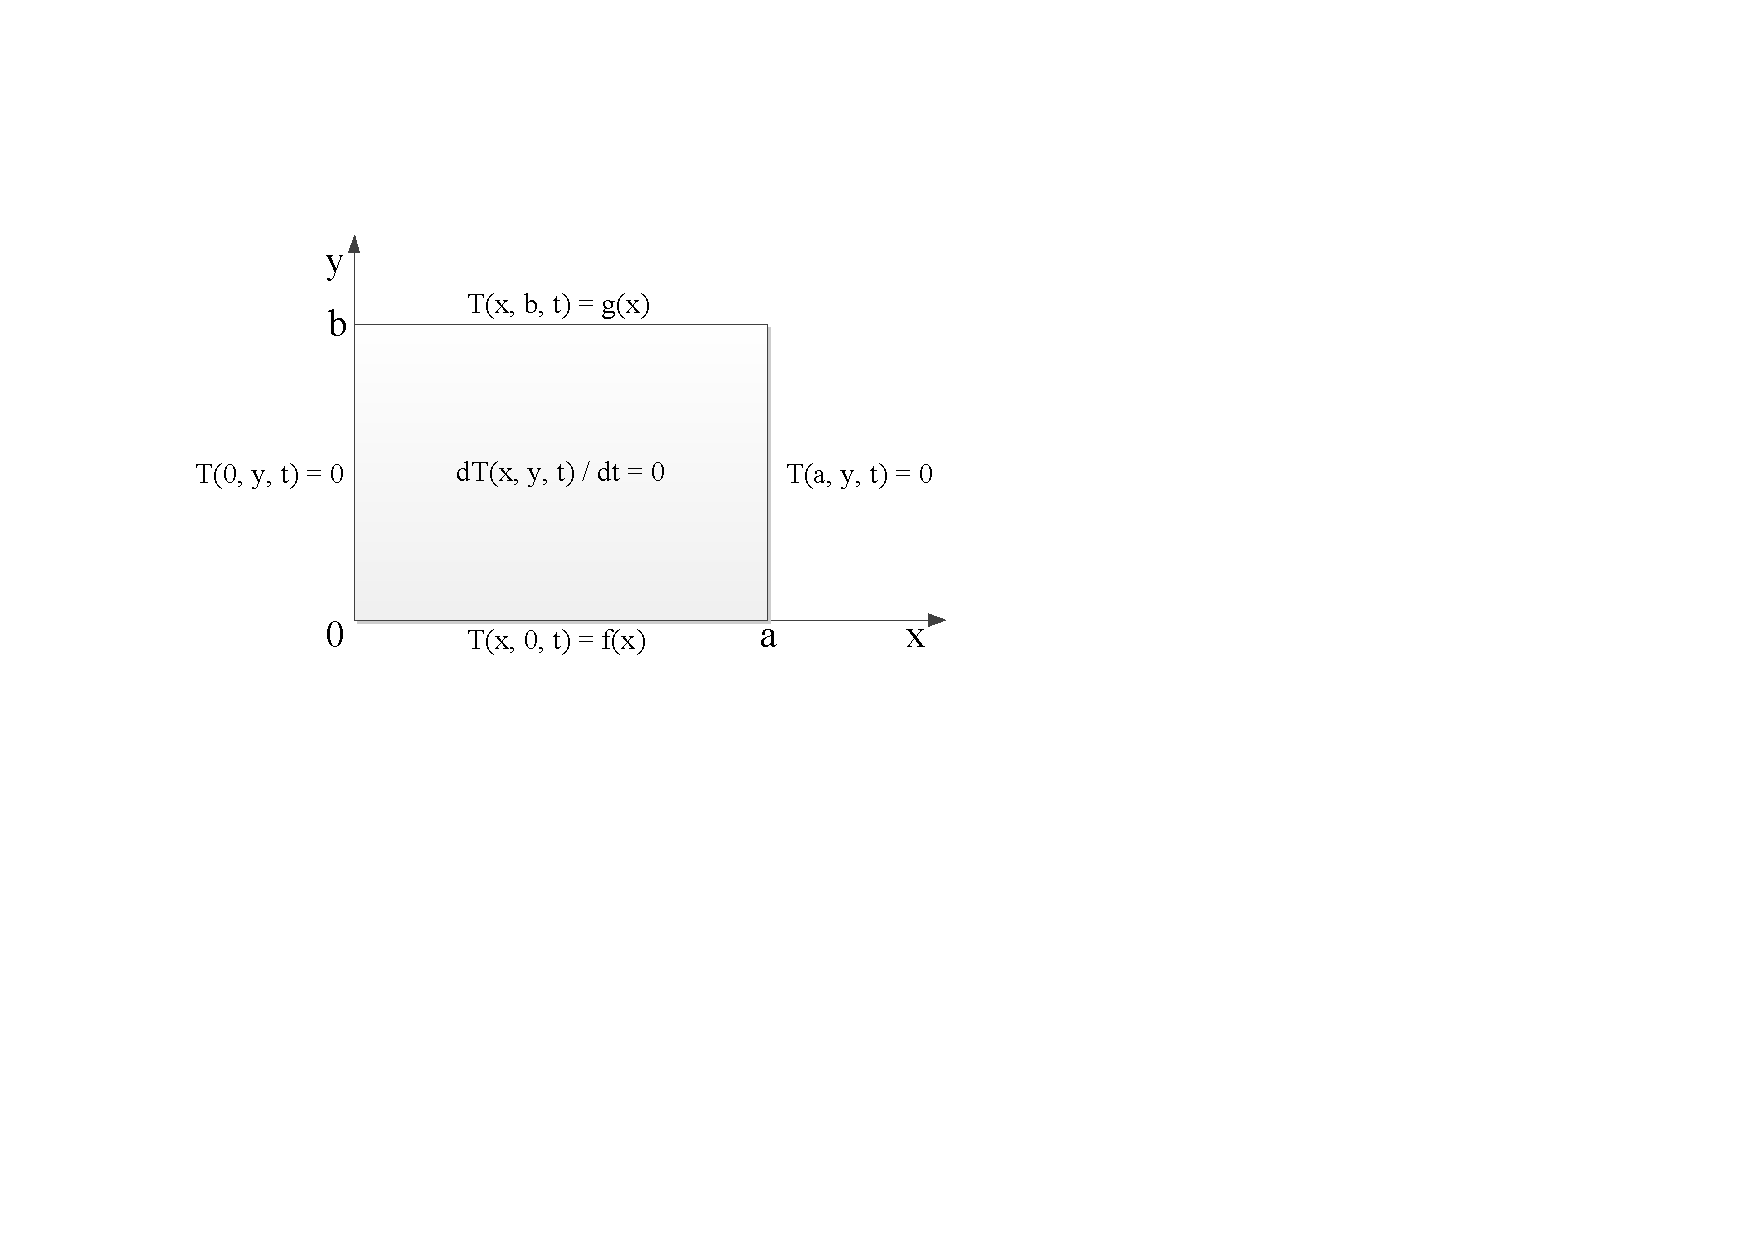
\includegraphics[width=10cm]{2dHeatSolDescription.pdf}       
	\caption{System description of the example}\label{heatSolSystem.fig}
\end{figure}

\paragraph{PDE and boundary conditions}
From Section 2.2.2 we have already known that the 2D heat equation is:
\begin{equation}
\frac{\partial T}{\partial t}=a^2\left(\frac{\partial ^2 T}{\partial x^2}+\frac{\partial ^2 T}{\partial y^2}\right)\ \ \ \ where\ a=\sqrt{\frac{k}{c\rho}}
\end{equation}


The boundary conditions of this problem are as follows:

\begin{equation}\label{2DHeatBound1.eq}
T(x,0,t)=f(x)
\end{equation}
\begin{equation}\label{2DHeatBound2.eq}
T(x,b,t)=g(x)
\end{equation}
\begin{equation}\label{2DHeatBound3.eq}
T(0, y, t)=0
\end{equation}
\begin{equation}\label{2DHeatBound4.eq}
T(a, y, t)=0
\end{equation}
\begin{equation}
\frac{\ud T}{\ud t}=0
\end{equation}

\paragraph{Solution}
Since the system is under the stationary state ($\ud T/\ud t=0$), $T(x,y,t)$ can be expressed as $T(x,y)$, and the PDE can be written as:
\begin{equation}
\frac{\partial^2T}{\partial x^2}+\frac{\partial^2T}{\partial y^2}=0
\end{equation}

We could sperate the variables by express $T(x,y)$ as $X(x)Y(y)$. Then the PDE can be written as:
\begin{equation}
X''(x)Y(y)+X(x)Y''(y)=0
\end{equation}

Since $X(x)Y(y)$ is not identically zero, divide both sides by $X(x)Y(y)$ gives:
\begin{equation}
\frac{X"(x)}{X(x)}+\frac{Y"(y)}{Y(y)}=0
\end{equation}

Since the two parts of the left side are independent, the following equations can be drawn ($\lambda$ is a constant):
\begin{align}
X"(x)+\lambda X(x)=0\\
Y"(y)-\lambda Y(y)=0
\end{align}

Moreover, the boundary conditions Equations~(\ref{2DHeatBound3.eq})-(\ref{2DHeatBound4.eq}) give:
\begin{align}
X(0)Y(y)=0\\
X(a)Y(y)=0
\end{align}

Since $Y(y)$ is not identically zero, we can obtain the following:
\begin{align}
X(0)=0\\
X(a)=0
\end{align}

Hence, the problem becomes solving two indenpendent ordinary differential equations. We know that only when $\lambda=\frac{n^2\pi^2}{a^2}\ (n=1,2,3,...)$, the problem has the following solution:
\begin{equation}
X_n(x)=sin\frac{n\pi x}{a}
\end{equation}
\begin{equation}
Y_n(y)=a_ne^{\frac{n\pi}{a}y}+b_ne^{-\frac{n\pi}{a}y}
\end{equation}

Hence, the solution can be expressed as:
\begin{equation}
T(x,y)=\sum_{n=1}^{\infty}(a_ne^{\frac{n\pi}{a}y}+b_ne^{-\frac{n\pi}{a}y})sin\frac{n\pi x}{a}
\end{equation}

Given the other two boundary conditions Equations~(\ref{2DHeatBound1.eq})-(\ref{2DHeatBound2.eq}), $a_n$ and $b_n$ can be solved using the following 2 equations:
\begin{equation}
a_n+b_n=\int_{0}^{a}f(x)sin\frac{n\pi}{a}xdx
\end{equation}
\begin{equation}
a_ne^{\frac{n\pi}{a}b}+b_ne^{-\frac{n\pi}{a}b}=\int_{0}^{a}g(x)sin\frac{n\pi}{a}xdx
\end{equation}

Thus, the analytical solution of this problem is solved.















